\documentclass[12pt, aspectratio=169]{beamer}
\usepackage[utf8]{inputenc}
\usepackage{amsmath, amssymb, amsthm, mathtools, gensymb, bm}
\usepackage{xcolor}
\usepackage{IEEEtrantools}
\setbeamercovered{transparent}
\newtheorem{prop}{Proposition}
\DeclarePairedDelimiter\ceil{\lceil}{\rceil}
\DeclarePairedDelimiter\floor{\lfloor}{\rfloor} % Ex: \floor*{\frac{x}{2}} < \frac{x}{2} < \ceil*{\frac{x}{2}}

\setbeamertemplate{footline}[frame number]
\setbeamertemplate{theorems}[numbered]
\beamertemplatenavigationsymbolsempty
\usecolortheme{seagull}
\usepackage{helvet}
\usefonttheme[onlymath]{serif}
\definecolor{alertcolor}{rgb}{.0, .48, .74}
\setbeamercolor{alerted text}{fg=alertcolor}

\newcommand{\trans}{\mathsf{T}}
\newcommand{\hermit}{\mathsf{H}}
\newcommand{\mc}[1]{\ensuremath{\mathcal{#1}}}
\newcommand{\mbb}[1]{\ensuremath{\mathbb{#1}}}
\newcommand{\Natural}{\mathbb{N}}
\newcommand{\Integer}{\mathbb{Z}}
\newcommand{\Irrational}{\mathbb{I}}
\newcommand{\Rational}{\mathbb{Q}}
\newcommand{\Real}{\mathbb{R}}
\newcommand{\Complex}{\mathbb{C}}
\newcommand{\obs}[1]{\textcolor{red}{(#1)}}
%\newcommand{\iff}{\mbox{$\Longleftrightarrow$}}    % biimplication
% \newcommand{\and}{\wedge}
% \newcommand{\or}{\vee}
\newcommand*\diff{\mathop{}\!\mathrm{d}}
\newcommand*\Diff[1]{\mathop{}\!\mathrm{d^#1}}
\newcommand{\ensureoperation}{\negmedspace {}} % To ensure that a new line symbol is an operation instead of a sign
\DeclarePairedDelimiter\abs{\lvert}{\rvert}%
\DeclarePairedDelimiter\norm{\lVert}{\rVert}%

% Swap the definition of \abs* and \norm*, so that \abs
% and \norm resizes the size of the brackets, and the 
% starred version does not.
% Usage example
% \abs{x} \norm{x}
% \abs*{x} \norm*{x}
\makeatletter
\let\oldabs\abs
\def\abs{\@ifstar{\oldabs}{\oldabs*}}
%
\let\oldnorm\norm
\def\norm{\@ifstar{\oldnorm}{\oldnorm*}}
\makeatother


\title{Homework 1 - MultiLinear Algebra}
\author{Rubem V. Pacelli}
\institute{Federal University of Ceará}
\date{\today}
 
\begin{document}
 
\frame[noframenumbering,plain]{\titlepage}

\begin{frame}[<+->][t]{Problem 01 - Item a}
	Let us define \(A,B \in \Complex^{N\times N}\). We have the following property
	\begin{IEEEeqnarray}{rCl}
		(A \otimes B)^{-1} = A^{-1} \otimes B^{-1}
		\label{eq:prop1}
	\end{IEEEeqnarray}
	\begin{visibleenv}<+->
		It important to notice the computational efficiency in both approach. Consider the task of calculating Eq.\eqref{eq:prop1} for \(N\in \left\{2, 4, 8, 16, 32, 64\right\}\).
	\end{visibleenv}
\end{frame}

\begin{frame}
	\frametitle{Problem 01 - Item a}
	\begin{figure}
		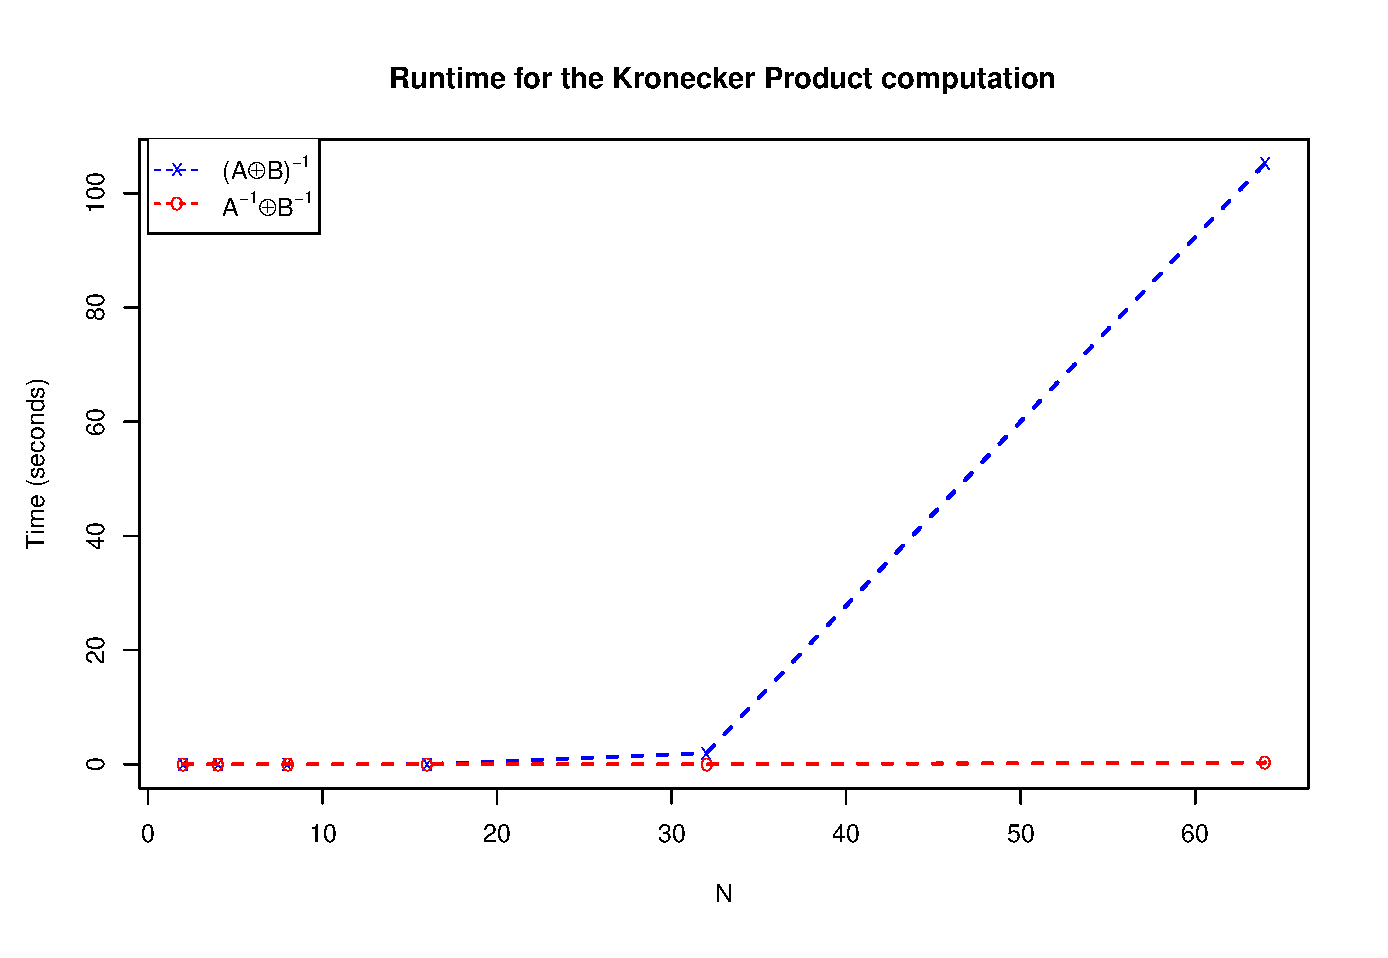
\includegraphics[scale=0.4]{figs/1a_norm.eps}
	\end{figure}
\end{frame}

\begin{frame}
	\frametitle{Problem 01 - Item a}
	\begin{figure}
		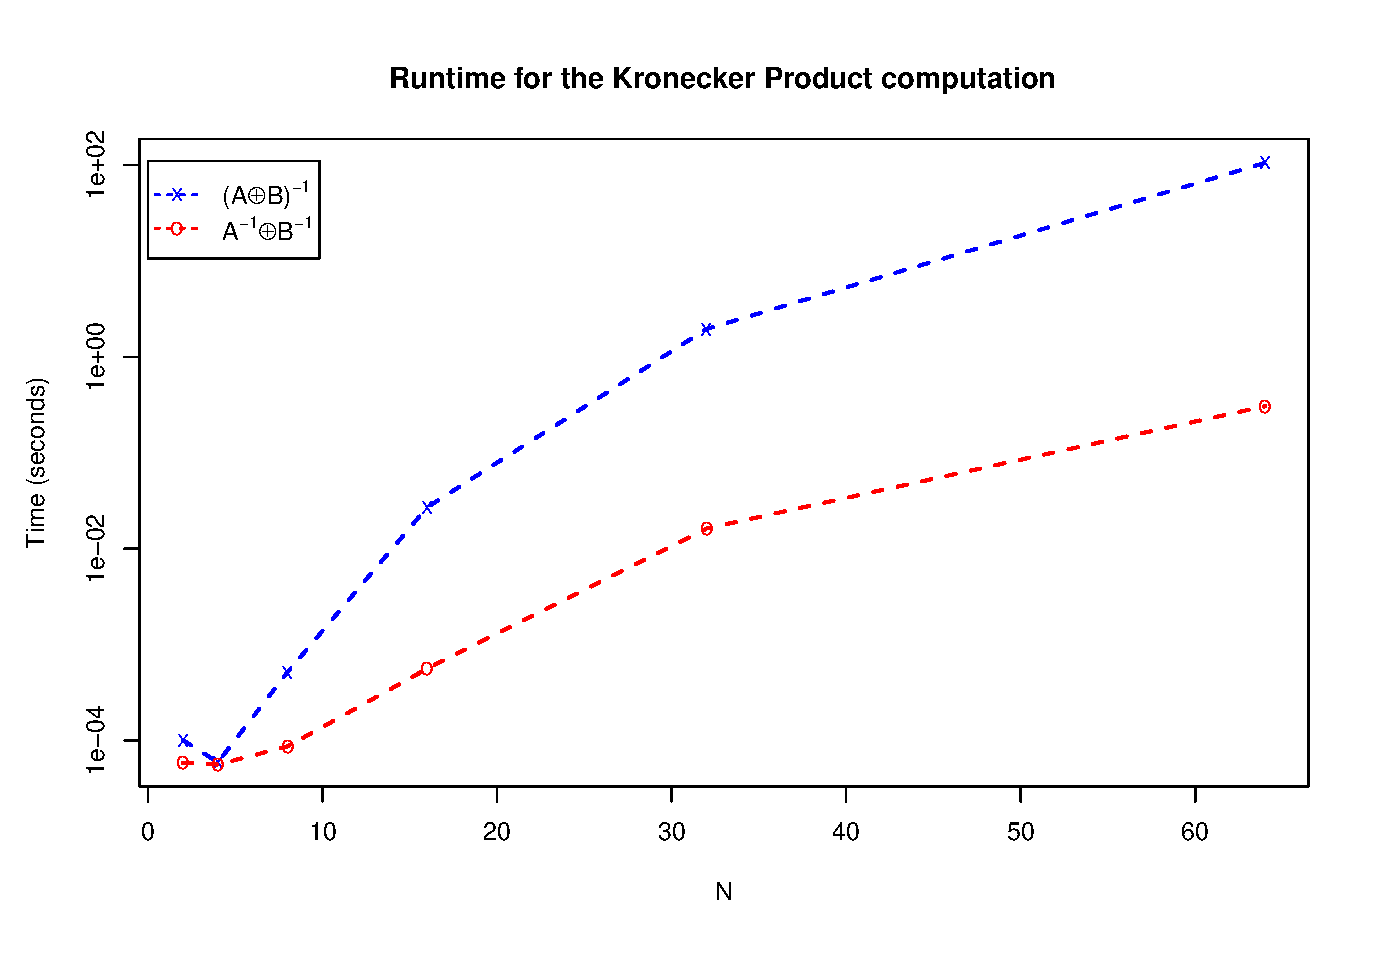
\includegraphics[scale=0.4]{figs/1a_log.eps}
	\end{figure}
\end{frame}

\begin{frame}
	\frametitle{Problem 01 - Item b}

	Now let us define \(N=2\) and vary the number of elements in the kronecker operation, that is
	\begin{IEEEeqnarray}{rCl}
		\left(\overset{k}{\underset{i=1}{\otimes}} A_{2\times2}\right)^{-1} = \overset{k}{\underset{i=1}{\otimes}} \left(A_{2\times2}\right)^{-1},
	\end{IEEEeqnarray}
	where \(k\in \left\{2,4,6,8,10\right\}\).

\end{frame}

\begin{frame}
	\frametitle{Problem 01 - Item b}
	\begin{figure}
		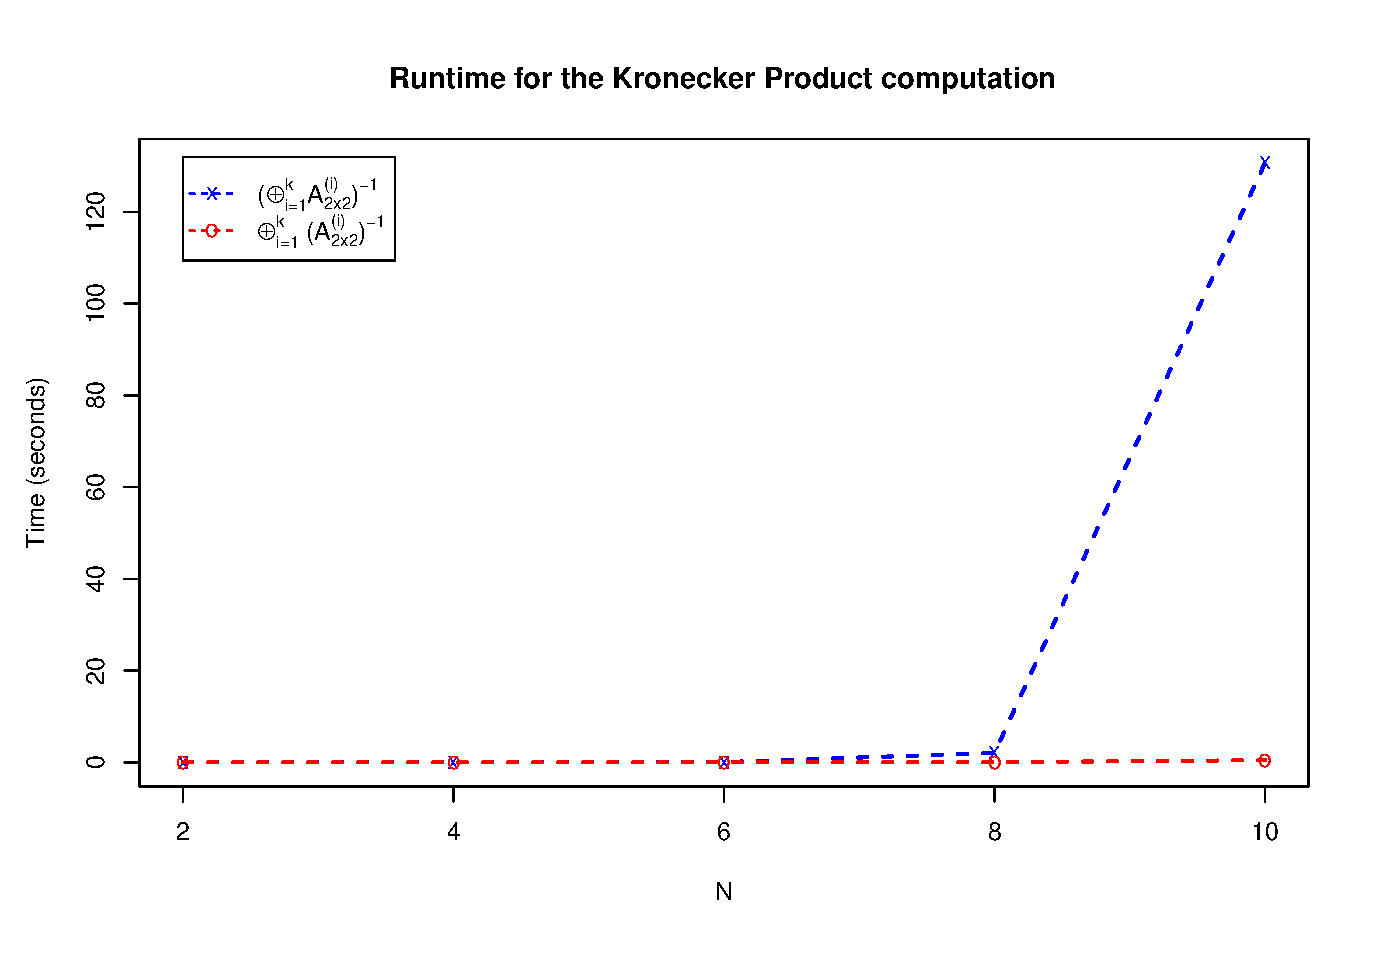
\includegraphics[scale=0.4]{figs/1b.eps}
	\end{figure}
\end{frame}

\begin{frame}
	\frametitle{Problem 01 - Item b}
	\begin{figure}
		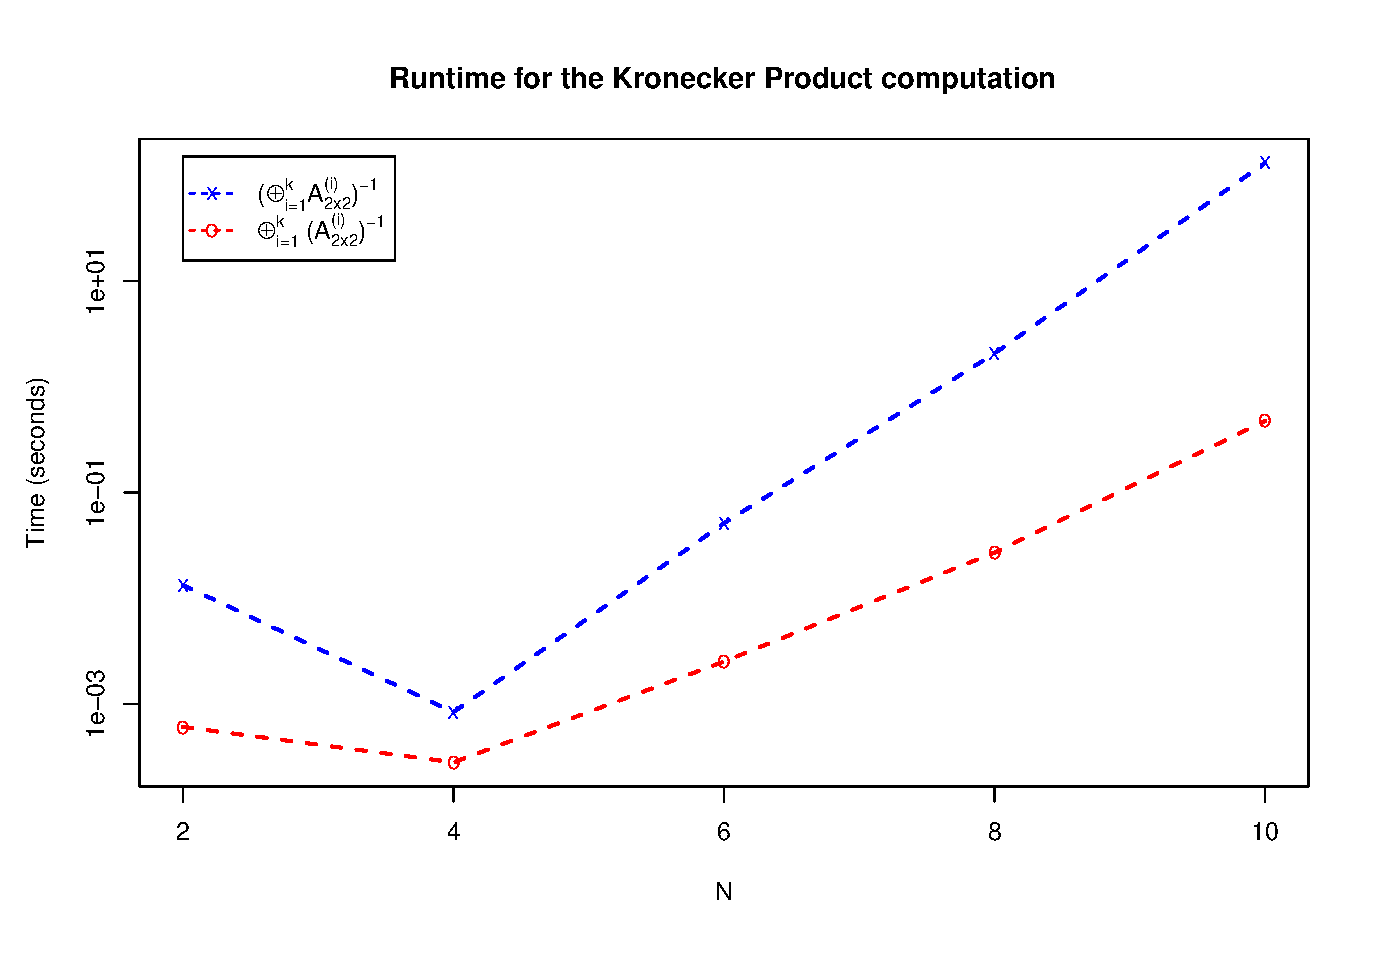
\includegraphics[scale=0.4]{figs/1b_log.eps}
	\end{figure}
\end{frame}

\begin{frame}[t]
	\frametitle{Problem 02}

	Proof that \(eig(\mathbf{A}\otimes \mathbf{B}) = eig(\mathbf{A}) \otimes eig(\mathbf{B})\). If \(\mathbf{A}\) and \(\mathbf{B}\) are diagonalizable and square matrices, the eigenvalues of \(\mathbf{A}\otimes\mathbf{B}\) is given by

	\begin{IEEEeqnarray}{rCl}
		\mathbf{A} \otimes \mathbf{B} &=& \mathbf{V}_A eig(A) \mathbf{V}_A^{-1} \otimes \mathbf{V}_B eig(B) \mathbf{V}_B^{-1} \\
									  &=& (\mathbf{V}_A \otimes\mathbf{V}_B)(eig(A) \otimes eig(B))(\mathbf{V}_A \otimes\mathbf{V}_B)^{-1} \\
									  &=& \mathbf{V}_{\mathbf{A}\otimes\mathbf{B}} eig(\mathbf{A}\otimes\mathbf{B}) \mathbf{V}_{\mathbf{A}\otimes\mathbf{B}}^{-1}
	\end{IEEEeqnarray}
	where \(\mathbf{V}_A\) and \(\mathbf{V}_B\) is the modal matrix of \(\mathbf{A}\) and \(\mathbf{B}\), respectively. It is possible to notice the que matrix containing the eigenvalues of \(\mathbf{A}\otimes\mathbf{B}\) is composed by the kronecker product of \(eig(A)\) and \(eig(B)\).s
\end{frame}

\end{document}